\label{es42}
\begin{flushleft}Il codice MatLab usato è il seguente:
\lstinputlisting[language=matlab]{cap_4/es2/es2.m}
Con $f(x) = \frac{1}{1+x^2}$ gli errori sono:
\[
\begin{tabu}{|c|c|c|c|}
\hline
n & Ascisse Equispaziate & Chebyshev \\
\hline
2 & 6.459699748665507\cdot10^{-1} & 6.005718959661196\cdot10^{-1} \\
4 & 4.382728746134097\cdot10^{-1} & 4.019561301268590\cdot10^{-1} \\
6 & 6.164015686420363\cdot10^{-1} & 2.641051307764343\cdot10^{-1} \\
8 & 1.045078216378144 & 1.700656314789976\cdot10^{-1} \\
10 & 1.915434269679889 & 1.090256419757498\cdot10^{-1} \\
12 & 3.611701597804764 & 6.902642915187807\cdot10^{-2} \\
14 & 7.189298472071057 & 4.608936896629207\cdot10^{-2} \\
16 & 1.401353448336841\cdot10 & 3.258023221036738\cdot10^{-2} \\
18 & 2.750677081179504\cdot10 & 2.212383276248159\cdot10^{-2} \\
20 & 5.840669034602058\cdot10 & 1.500717452472311\cdot10^{-2} \\
\hline
\end{tabu}
\]
Il grafico ottenuto per questa funzione con n=6 è:
\begin{figure}[H]
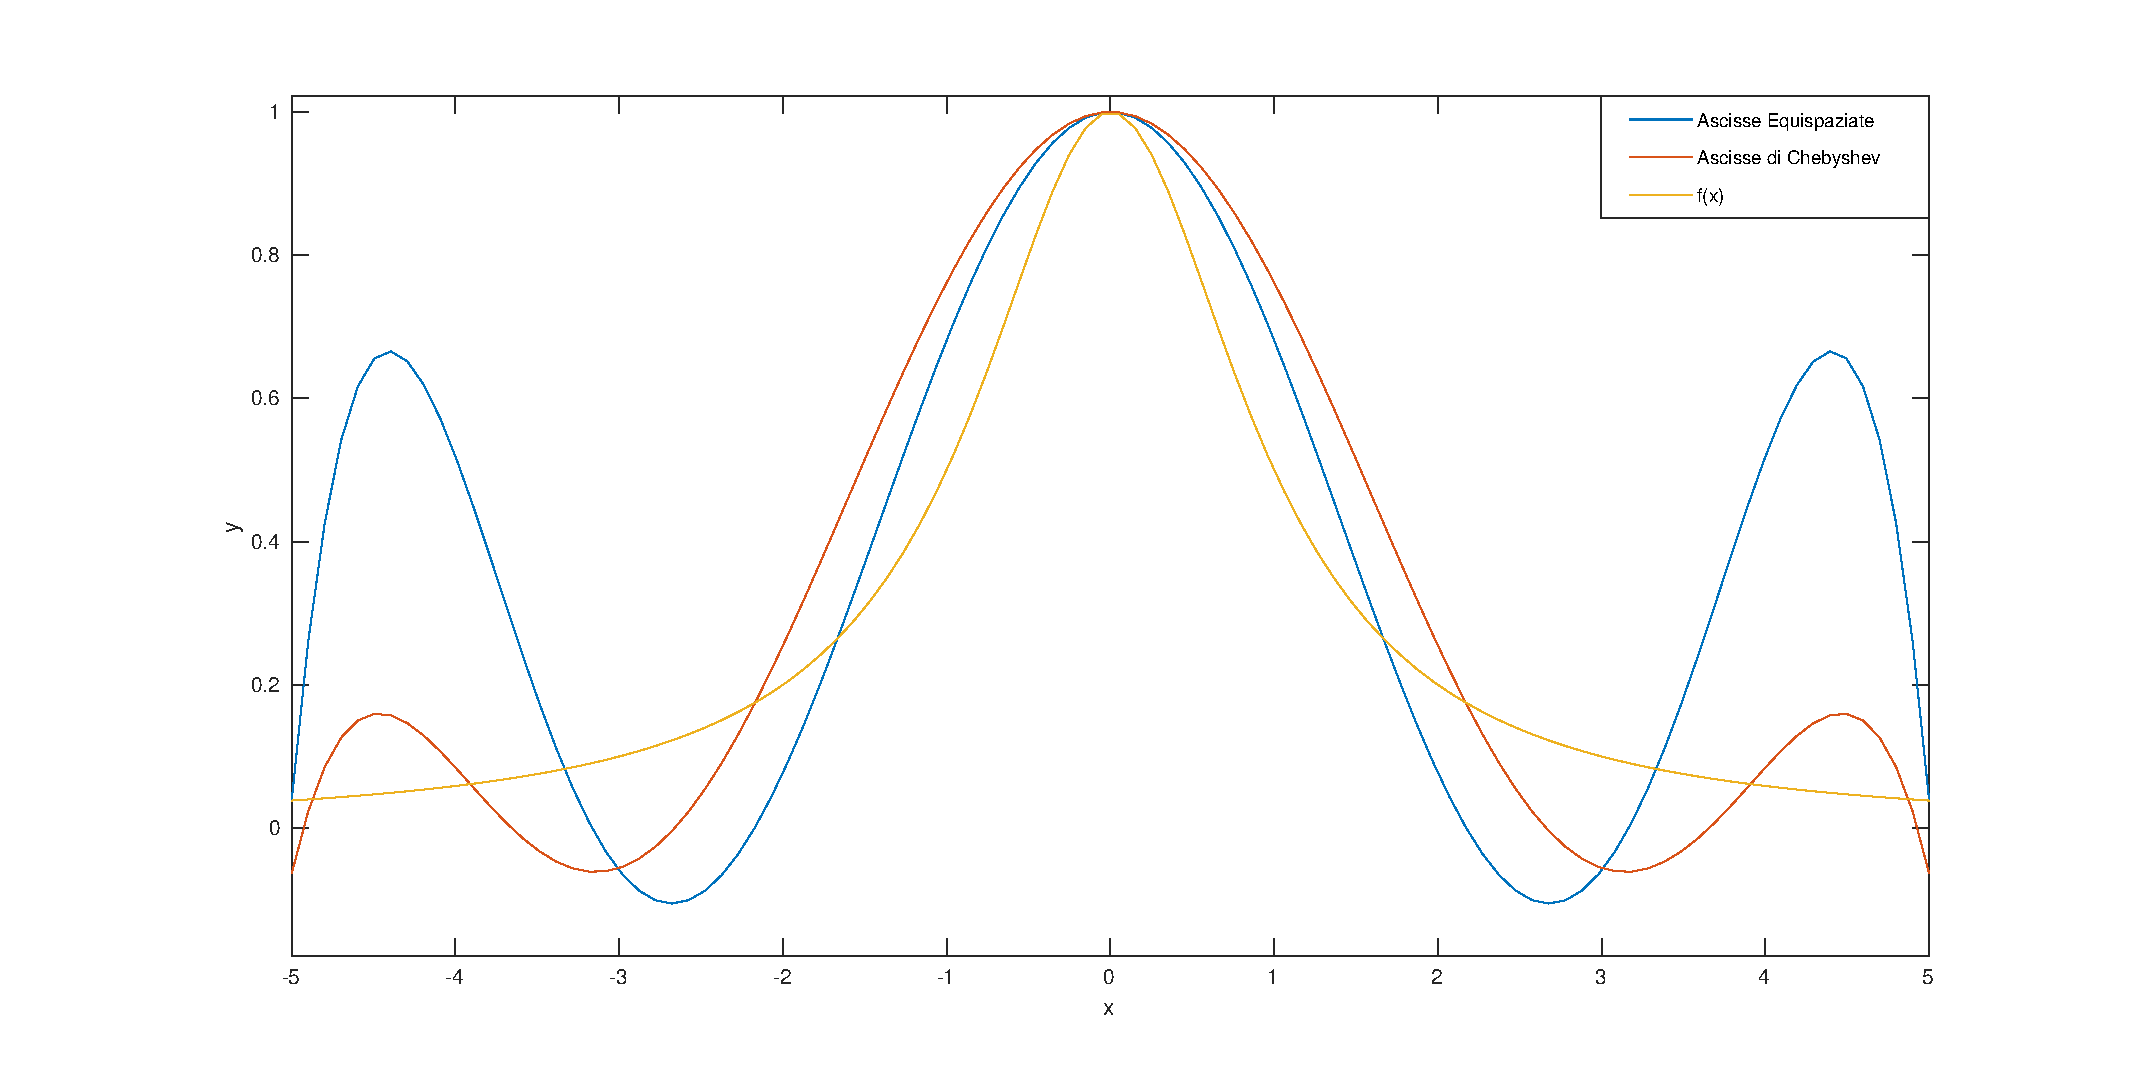
\includegraphics[width=480px, height=280px]{plot/fes42a}
\caption{\texttt{Confronto tra il grafico reale della funzione e le rispettive interpolazioni}}
\end{figure}
\newpage
Il grafico ottenuto per questa funzione con n=12 è:
\begin{figure}[H]
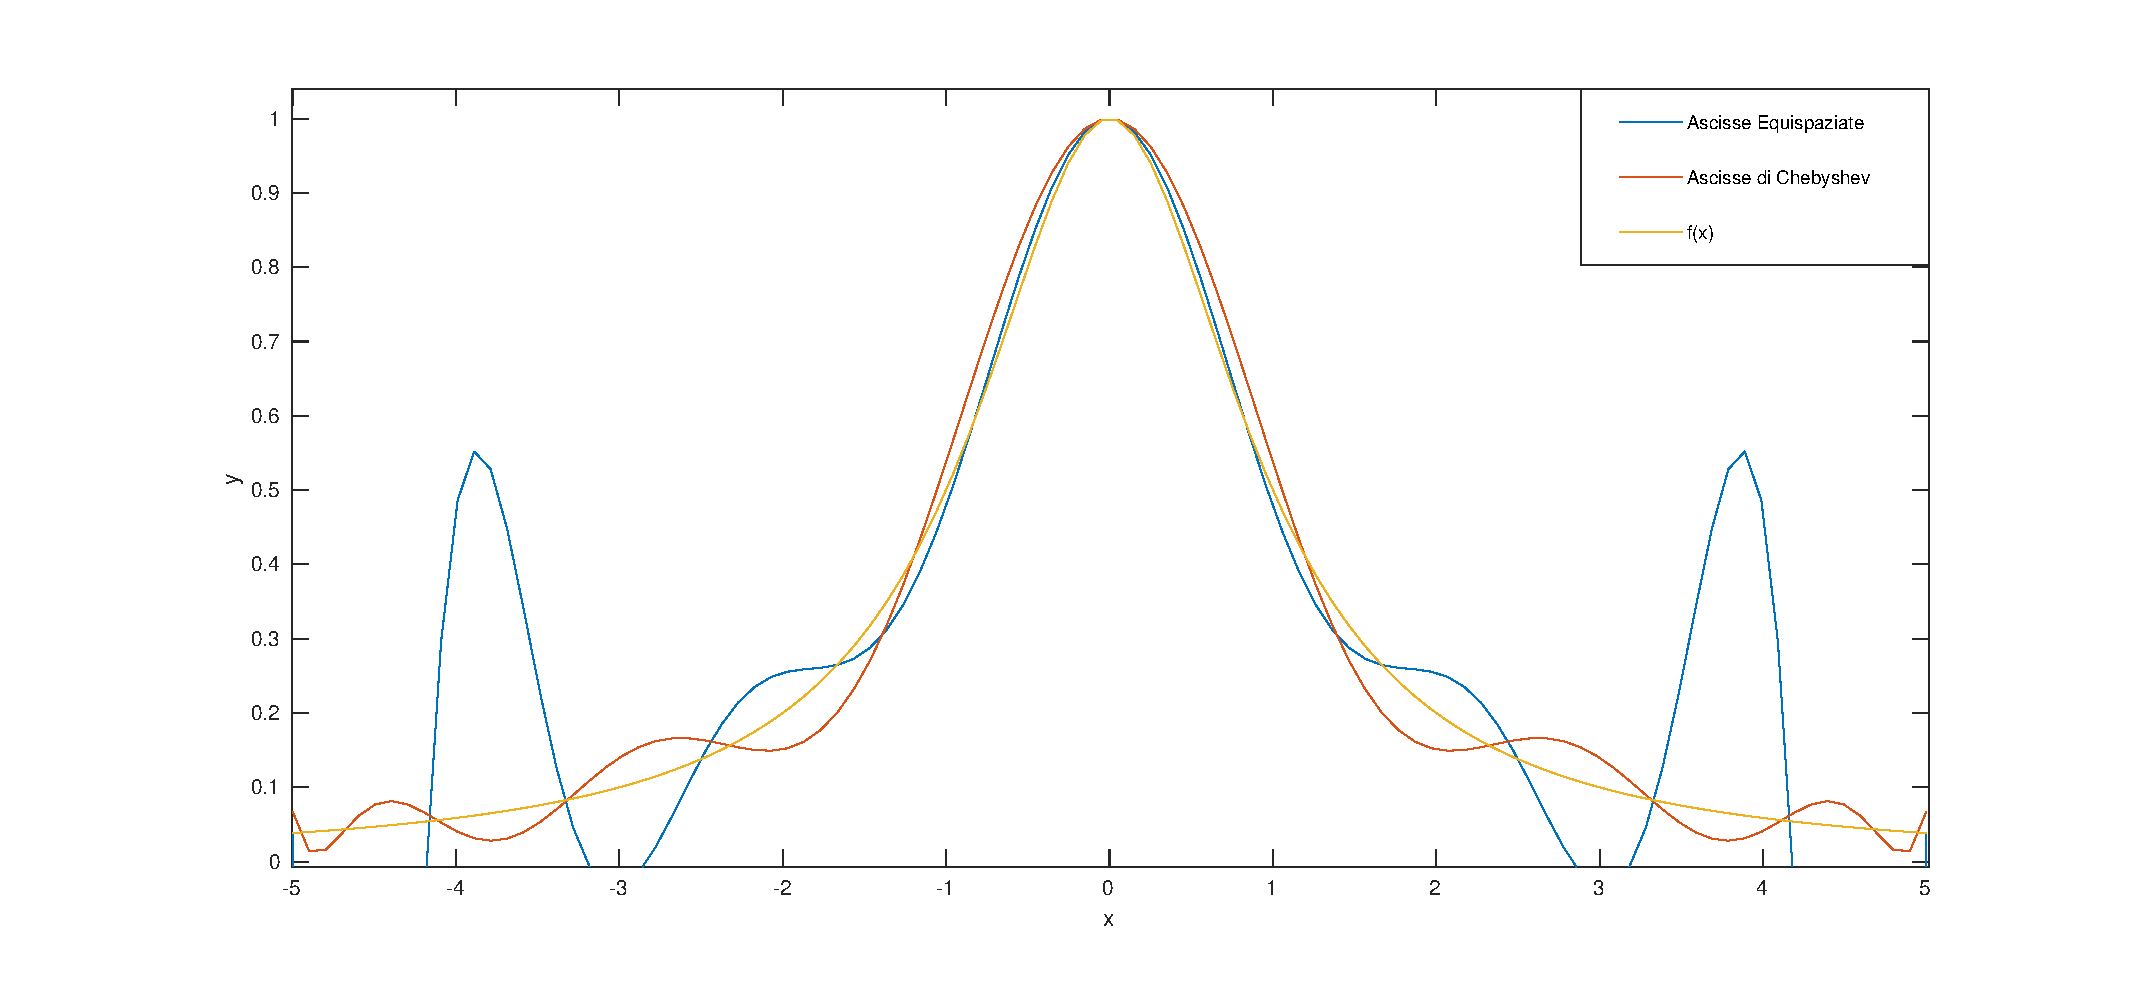
\includegraphics[width=480px, height=280px]{plot/fes42d}
\caption{\texttt{Confronto tra il grafico reale della funzione e le rispettive interpolazioni}}
\end{figure}
Nel caso in cui $f(x) = x\cdot sin(x)$ gli errori sono:
\[
\begin{tabu}{|c|c|c|c|}
\hline
i & Ascisse Equispaziate & Chebyshev \\
\hline
2 & 6.381422078133654\cdot10^{-1} & 4.370888339682153\cdot10^{-1}\\
4 & 4.127250365828502\cdot10^{-2} & 2.286331189343005\cdot10^{-2}\\
6 & 1.343141368041964\cdot10^{-3} & 4.779185850743994\cdot10^{-4}\\
8 & 2.575400820072765\cdot10^{-5} & 5.331729223456705\cdot10^{-6}\\
10 & 3.237670194583542\cdot10^{-7} & 3.688279803792938\cdot10^{-8}\\
12 & 2.843434354291019\cdot10^{-9} & 1.733829746441984\cdot10^{-10}\\
14 & 1.873067152768915\cdot10^{-11} & 5.891953591685706\cdot10^{-13}\\
16 & 1.261490911730334\cdot10^{-13} & 3.417152747496221\cdot10^{-15}\\
18 & 8.933132011890166\cdot10^{-14} & 1.776356839400250\cdot10^{-15}\\
20 & 1.768307722471718\cdot10^{-13} & 2.327007791852781\cdot10^{-15}\\
\hline
\end{tabu}
\]
\newpage
Il grafico per questa funzione con n=2 è il seguente:
\begin{figure}[H]
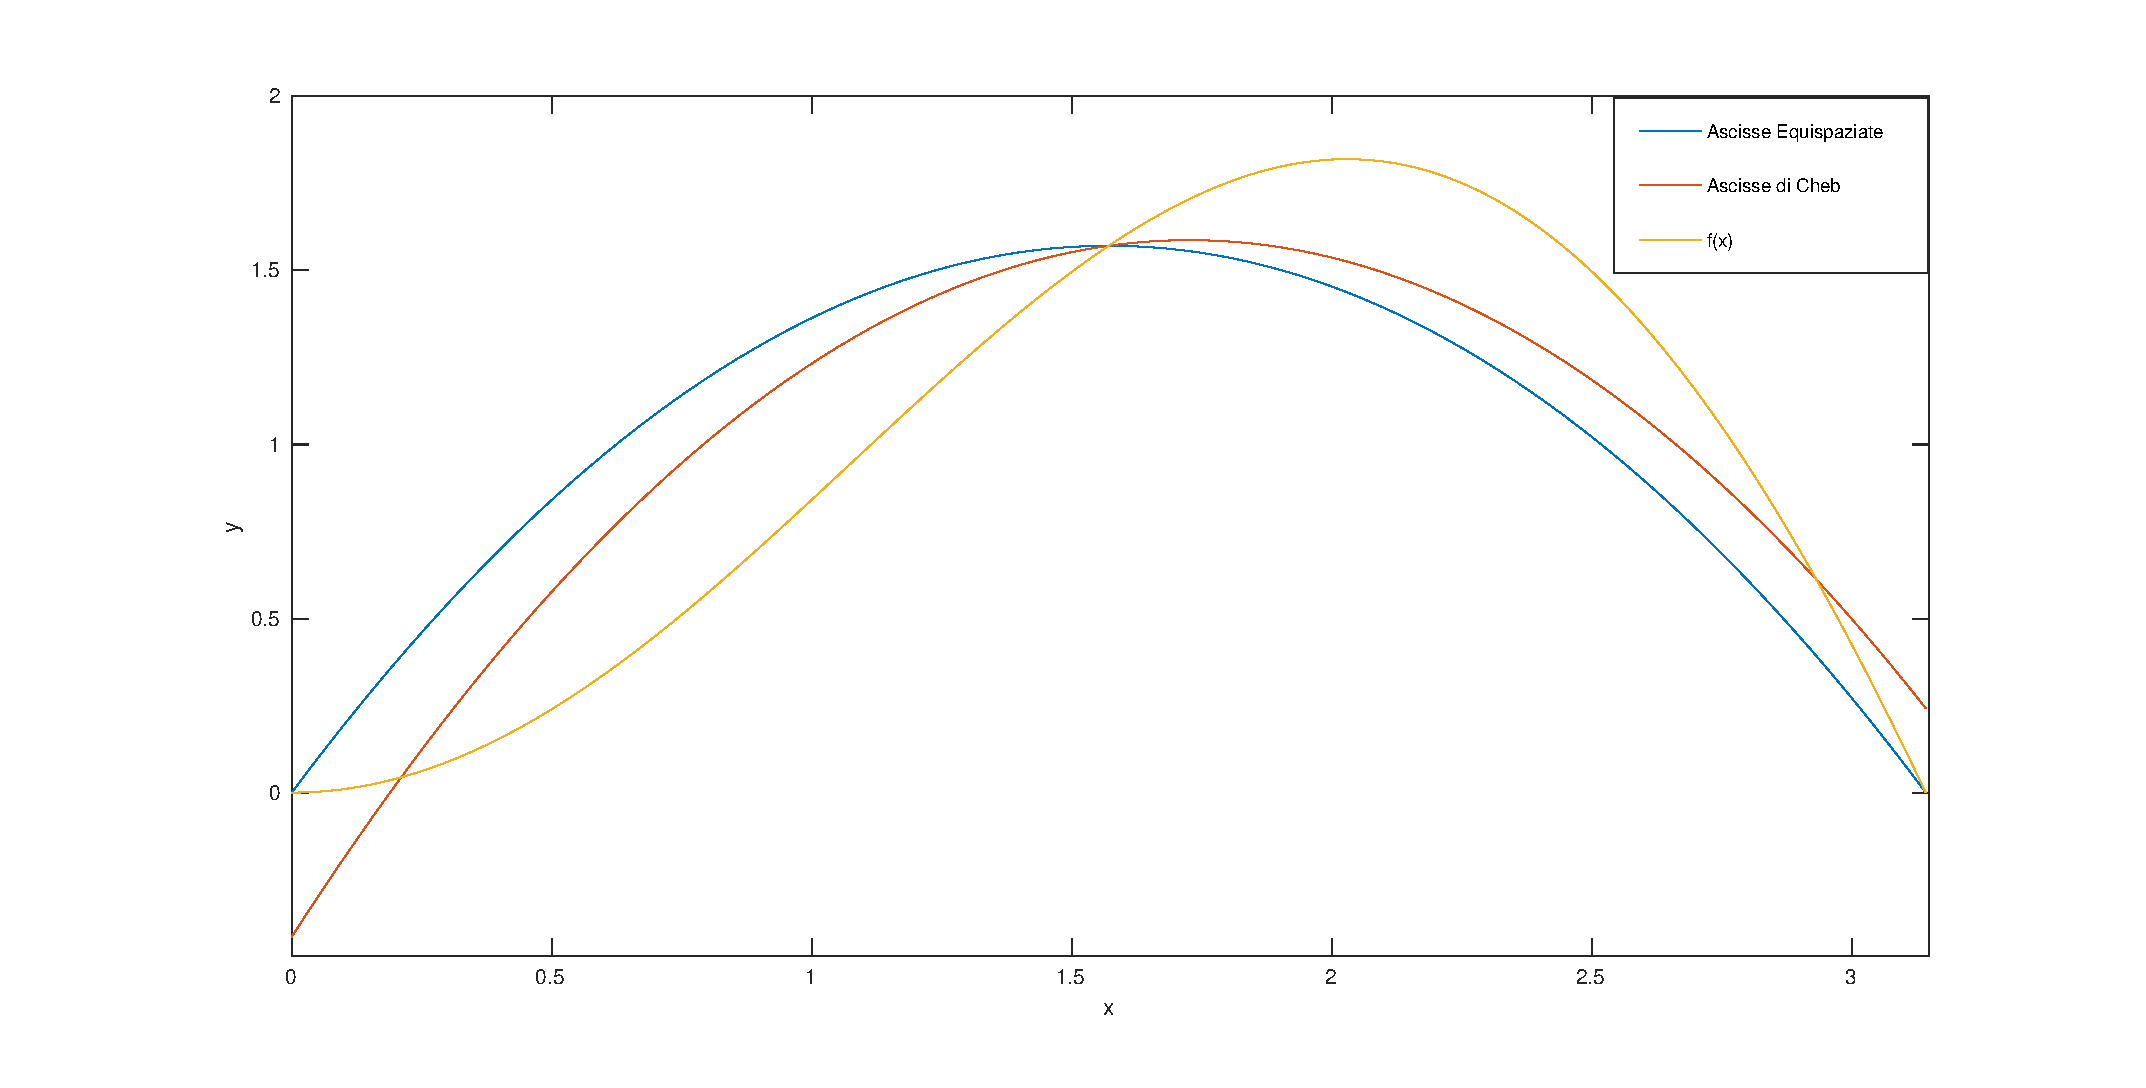
\includegraphics[width=480px, height=280px]{plot/fes42b}
\caption{\texttt{Confronto tra il grafico reale della funzione e le rispettive interpolazioni}}
\end{figure}
Il grafico per questa funzione con n=4 è il seguente:
\begin{figure}[H]
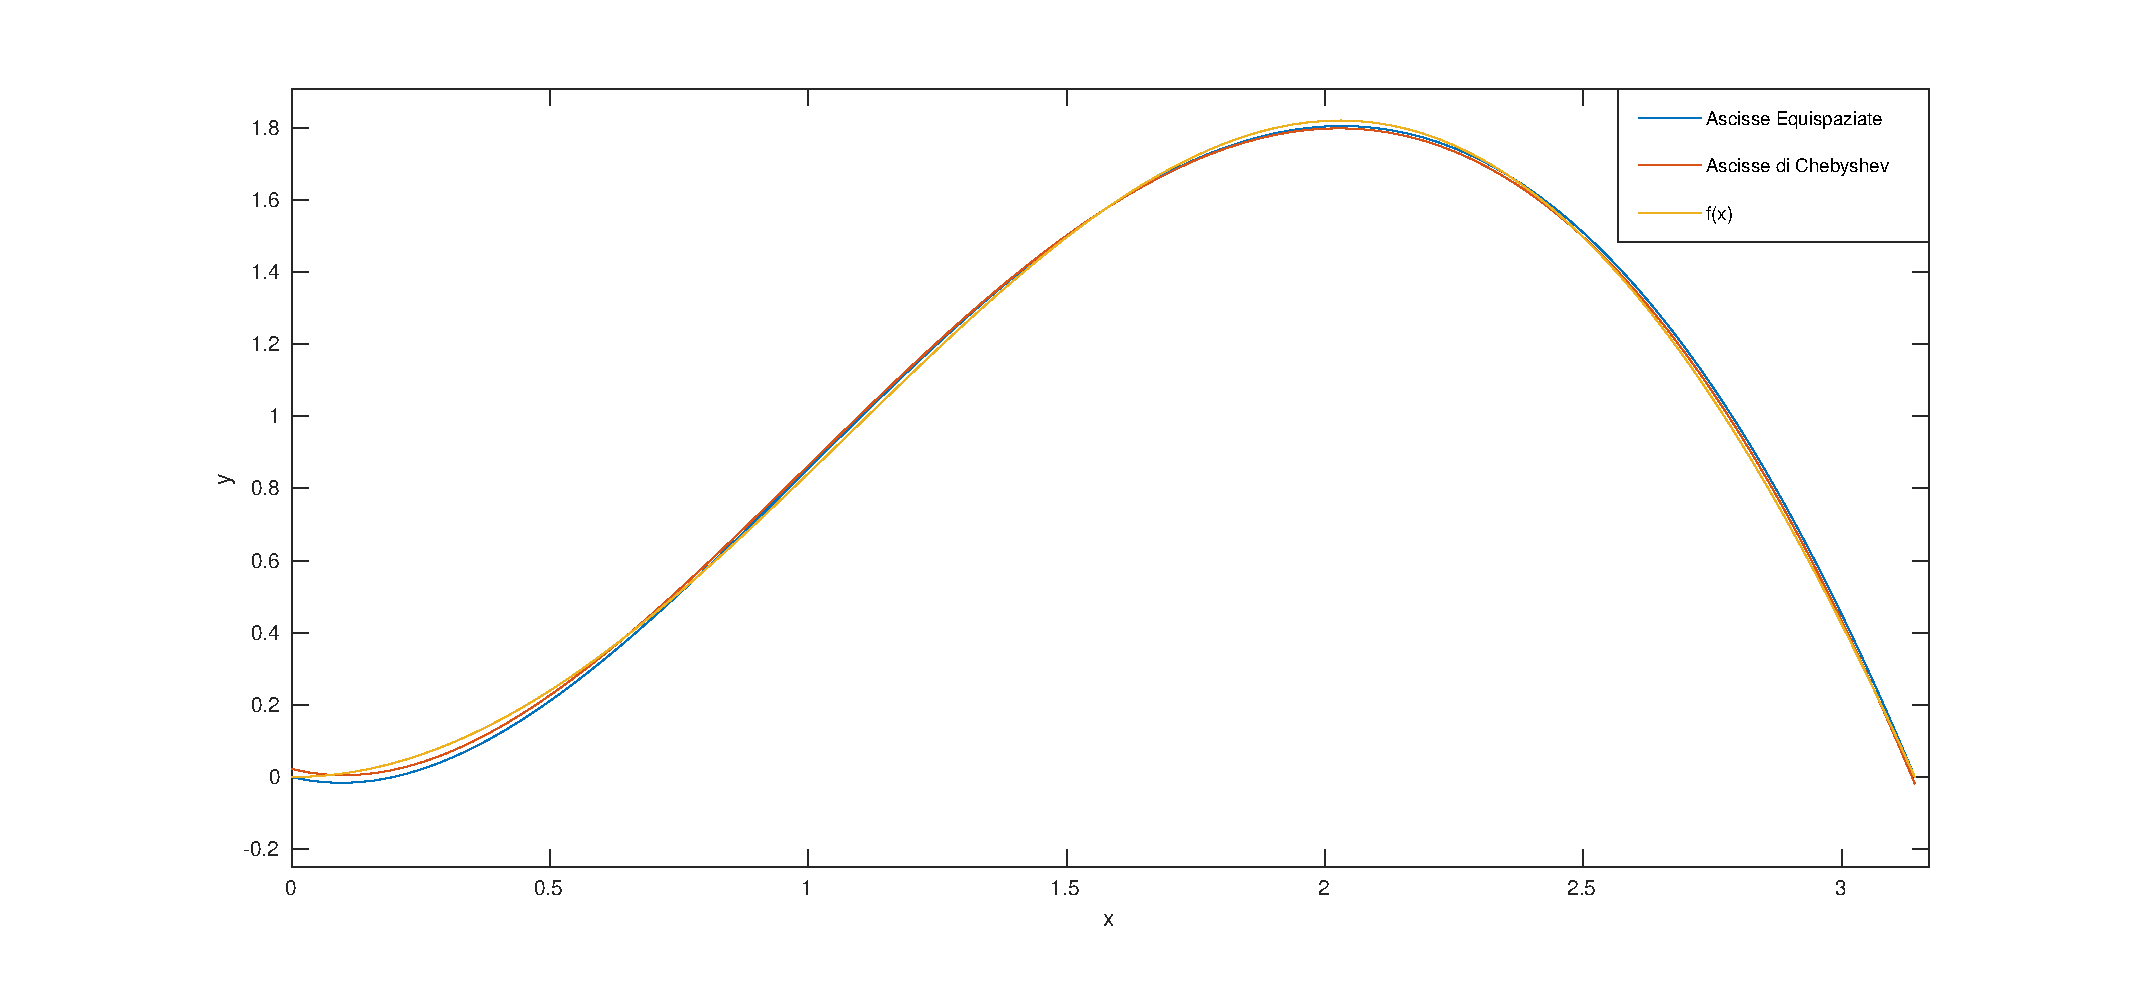
\includegraphics[width=480px, height=280px]{plot/fes42c}
\caption{\texttt{Confronto tra il grafico reale della funzione e le rispettive interpolazioni}}
\end{figure}
Si può vedere dai 2 grafici che le due interpolazioni all'aumentare di n si avvicinano al reale grafico di $f(x)=x\cdot sin(x)$. Con $n=20$ si arriva ad un errore relativo dell'ordine di $10^{-13}$ e $10^{-15}$, cioè un'interpolazione ottima della funzione originaria.
\end{flushleft}